\documentclass[12pt]{standalone}

\usepackage{tikz}
\usetikzlibrary{shapes,arrows,decorations.pathreplacing}


\tikzstyle{bs_block}=[right,yshift=0.5cm,rectangle,draw=black!60, thick, inner sep=0pt, minimum size=1cm, minimum height=0.8cm]
\tikzstyle{axis} = [->,thick,>=stealth']
\tikzstyle{arrow} = [->,thin,>=stealth']
\tikzstyle{ss_block} = [right,rectangle,draw=black!60, thick, inner sep=0pt, minimum size=0.1cm, minimum height=0.5cm, fill=blue!50]
\tikzstyle{csi_block} = [right,rectangle,draw=black!60, thick, inner sep=0pt, minimum size=0.1cm, minimum height=0.2cm, fill=red!50]

\begin{document}

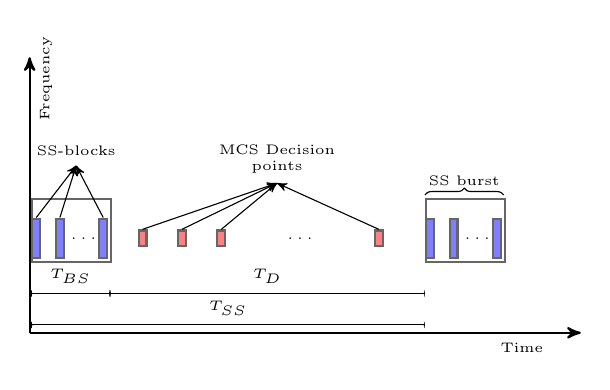
\begin{tikzpicture}

\coordinate (ref) at (0,0);
\coordinate (A) at (7,0);
\coordinate (B) at (0,3.5);
\coordinate (A2) at (5,0);

\node[bs_block,yshift=0.8cm,xshift=0.02cm] (initial)  at (ref) {};
\node[ss_block,xshift=0.02cm,yshift=1.2cm] (first_ss)   at (ref) {};
\node[ss_block] (second_ss)  [right of=first_ss,xshift=-0.7cm] {};
\node[] (dots) [right of=second_ss,xshift=-0.7cm] {\tiny{$\ldots$}};
\node[ss_block] (third_ss)  [right of=dots,xshift=-0.75cm] {};
\node[]  (text_one)  [above right of = first_ss,yshift=0.4cm,xshift=-0.2cm] {\tiny{SS-blocks}};
\draw[arrow] (first_ss.north)  -- (text_one.south);
\draw[arrow] (second_ss.north)  -- (text_one.south);
\draw[arrow] (third_ss.north)  -- (text_one.south);


\node[bs_block,yshift=0.8cm,xshift=0.02cm] (second)   at (A2) {};
\node[ss_block,xshift=0.02cm,yshift=1.2cm] (first2_ss)   at (A2) {};
\node[ss_block] (second2_ss)  [right of=first2_ss,xshift=-0.7cm] {};
\node[] (dots) [right of=second2_ss,xshift=-0.7cm] {\tiny{$\ldots$}};
\node[ss_block] (third2_ss)  [right of=dots,xshift=-0.75cm] {};
\draw[<->,>=serif cm] (0.02cm,0.5cm) -- ++(1,0) node [midway, above] {\tiny{$T_{BS}$}};
\draw[<->,>=serif cm] (1.02cm,0.5cm) -- ++(4,0) node [midway, above] {\tiny{$T_{D}$}};
\draw[<->,>=serif cm] (0.02cm,0.1cm) -- ++(5,0) node [midway, above] {\tiny{$T_{SS}$}};


\draw[axis] (ref) -- (A) node [near end, below, xshift=1cm] {\tiny{Time}};
\draw[axis] (ref) -- (B) node [near end, below,rotate=90,xshift=0.6cm] {\tiny{Frequency}};

\draw[decorate,decoration=brace,yshift=1.75cm, xshift=0.02cm]
(5,0) -- (6,0) node [black,midway,above] {\tiny{SS burst}};

\node[csi_block] (first_csi) [right of=third_ss,xshift=-0.5cm] {};
\node[csi_block] (second_csi) [right of=first_csi,xshift=-0.5cm] {};
\node[csi_block] (third_csi) [right of=second_csi,xshift=-0.5cm] {};
\node[] (dots_csi) [right of=third_csi,xshift=0] {\tiny{$\ldots$}};
\node[csi_block] (fourth_csi) [right of=dots_csi,xshift=0cm] {};
\node[]  (text_two)  [above right of = first_csi,yshift=0.3cm,xshift=1cm] {\parbox{1.5cm}{\tiny \centering MCS Decision \\ points}};
\draw[arrow] (first_csi.north)  -- (text_two.south);
\draw[arrow] (second_csi.north)  -- (text_two.south);
\draw[arrow] (third_csi.north)  -- (text_two.south);
\draw[arrow] (fourth_csi.north)  -- (text_two.south);
\end{tikzpicture}

\end{document}
